%%-*-latex-*-

% ------------------------------------------------------------------------
%
\begin{frame}
\frametitle{Trees}

At this point it is important to understand the two usages of the
word \emph{tree}. 

\bigskip

We introduced a map between terms and trees, because this new point of
view gives  some insights  (e.g. the \({\cal H}\) function).  In this
context,  a tree  is  another \textbf{representation}  of the  subject
(terms) we are studying, it is a tool.

\bigskip

But this section now presents trees as a \textbf{data structure} on
its own. In this context, a tree is the subject of our study, they are
given. This is why, when studying the stacks (the subject), we
displayed them as trees (an intuitive graphics representation).

\end{frame}

% ------------------------------------------------------------------------
%
\begin{frame}
\frametitle{Tree traversals}

Given a tree, we can traverse it in many ways, but we must start from
the root since we do not have any other node at this level. There are
two main kind of traversals:
\begin{itemize}

  \item \textbf{Breadth-first} traversal consists in walking the
  tree by increasing levels: first the root (level 0), the sons of the
  root (level 1), then the sons of the sons (level 2) etc. 

  \item \textbf{Depth-first} traversal consists in walking the tree 
  by reaching the leaves as soon as possible.

\end{itemize}
In both cases, we are finished when all the leaves have been encountered.

\end{frame}

% ------------------------------------------------------------------------
%
\begin{frame}
\frametitle{Tree traversals/Breadth-first}

\label{breadth_first_pictures}

Let us consider two examples of breadth-first traversals.

\bigskip

\begin{columns}
  \column{0.5\textwidth}
    \begin{center}
      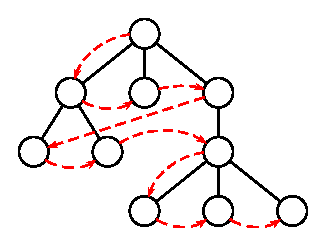
\includegraphics[bb=71 619 211 721]{breadth-first_1}
    \end{center}
    This is a \textbf{left to right} traversal.
  \column{0.5\textwidth}
    \begin{center}
      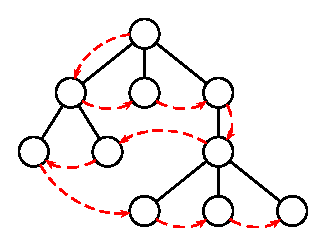
\includegraphics[bb=71 619 211 721]{breadth-first_2}
    \end{center}
\end{columns}

\bigskip

Many others are possible, like choosing randomly the next node of the
following level.

\end{frame}

% ------------------------------------------------------------------------
%
\begin{frame}
\frametitle{Tree traversals/Depth-first}

Let us consider two examples of depth-first traversals.

\bigskip

\begin{columns}
  \column{0.5\textwidth}
    \begin{center}
      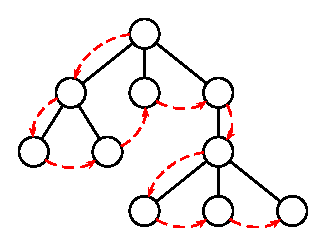
\includegraphics[bb=71 619 211 721]{depth-first_1}
    \end{center}
    This is a \textbf{left to right} traversal.
  \column{0.5\textwidth}
    \begin{center}
      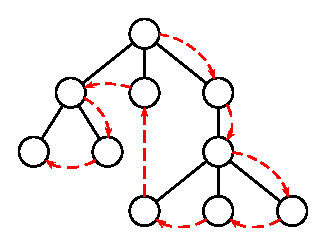
\includegraphics[bb=71 619 211 721]{depth-first_2}
    \end{center}
    This is a \textbf{right to left} traversal.
\end{columns}

\end{frame}

% ------------------------------------------------------------------------
%
\begin{frame}
\frametitle{Binary trees}

In order to simplify, let us consider here trees with two direct
subtrees. They are called \textbf{binary trees}. We do not lose
generality with this restriction: it is always possible to map any
tree to a binary tree in a unique way: the \textbf{left son, right
brother} technique:
\begin{center}
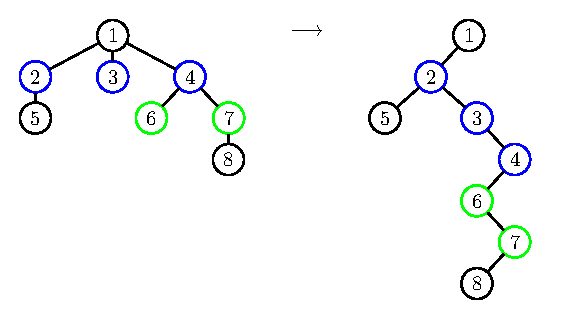
\includegraphics[bb=71 584 317 721]{left_brother}
\end{center}

\end{frame}

% ------------------------------------------------------------------------
%
\begin{frame}
\frametitle{Binary trees/Signature}

Let us formally define a a binary tree and call it \(\proc{Bin-tree}
(\type{node})\), where \type{node} is the type of the nodes. Here is
the \textbf{signature}:
\begin{itemize}

  \item \textbf{Parameter types}

  \begin{itemize}
 
     \item The type \type{node} of the nodes.

  \end{itemize}

  \item \textbf{Defined types}

    \begin{itemize}

      \item The type of the binary trees is \type{t}.
    
  \end{itemize}

  \item \textbf{Constructors}

   \begin{itemize}

     \item \(\proc{Empty} : \type{t}\)\\ The constant \proc{Empty} is
       the empty tree (it is a constant function).

     \item \(\proc{Make} : \type{node} \times \type{t} \times \type{t}
       \rightarrow \type{t}\)\\ The tree \(\proc{Make} (\id{n},
       \id{t_1}, \id{t_2})\) as root \id{n} and
       subtrees \id{t_1} and \id{t_2}.

   \end{itemize}

\end{itemize}

\end{frame}

% ------------------------------------------------------------------------
%
\begin{frame}
\frametitle{Binary trees/Signature (cont)}

Let us show some examples of tree construction:
\[
{\scriptsize
\begin{array}{c|c}
  \proc{Empty} 
& \varnothing\\
\hline
  \proc{Make} (\id{n_1}, \proc{Empty}, \proc{Empty})
& 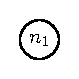
\includegraphics[bb=71 701 91 721]{n1}\\%[8pt]
\hline
  \proc{Make} (\id{n_1}, \proc{Empty}, \proc{Make} (\id{n_2},
  \proc{Empty}, \proc{Empty}))
& 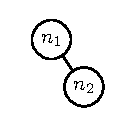
\includegraphics[bb=77 678 112 721]{n1_n2}\\%[10mm]
\hline
  \proc{Make} (\id{n_1}, \proc{Make} (\id{n_3},
  \proc{Empty}, \proc{Empty}), \proc{Make} (\id{n_2},
  \proc{Empty}, \proc{Empty}))
& 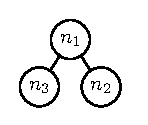
\includegraphics[bb=71 678 120 721]{n1_n2_n3}
\end{array}
}
\]

\end{frame}

% ------------------------------------------------------------------------
%
\begin{frame}
\frametitle{Binary trees/Signature (cont)}

The only projection for binary trees is the reverse function for
\proc{Make}: \[\proc{Make}^{-1} \circ \proc{Make} = \id{id}\] where
\id{id} is the identity function. In other words \[\forall \id{n},
\id{t_1}, \id{t_2} \quad \proc{Make}^{-1} (\proc{Make} (\id{n},
\id{t_1}, \id{t_2})) = (\id{n}, \id{t_1}, \id{t_2})\]

We gave no name to the reverse of \proc{Make} because \((\id{n},
\id{t_1}, \id{t_2})\) does not correspond to a well-identified
concept. Then let us choose more intuitive projections.

\end{frame}

% ------------------------------------------------------------------------
%
\begin{frame}
\frametitle{Binary trees/Signature (cont)}

\begin{itemize}

  \item \textbf{Projections}
  
 \begin{itemize}

    \item \(\proc{Make}^{-1} : \type{t} \rightarrow \type{node}
    \times \type{t} \times \type{t}\)\\
    This is the inverse function of constructor \proc{Make}.

    \item \(\proc{Root} : \type{t} \rightarrow
      \type{node}\)\\ Expression \(\proc{Root} (\id{t})\) represents
      the root of tree \id{t}.

    \item \(\proc{Left} : \type{t} \rightarrow \type{t}\)\\ Expression
      \(\proc{Left} (\id{t})\) denotes the left subtree of tree
      \id{t}.

    \item \(\proc{Right} : \type{t} \rightarrow \type{t}\)\\
    Expression \(\proc{Right} (\id{t})\) denotes the right subtree of
    tree \id{t}.

 \end{itemize}

\end{itemize}

\end{frame}

% ------------------------------------------------------------------------
%
\begin{frame}
\frametitle{Binary trees/Equations}

As we guessed with the case of \(\proc{Make}^{-1}\), we can complement
our signature using \textbf{equations} (or \textbf{axioms}):
\[
\begin{aligned}
&\forall \id{n}, \id{t_1}, \id{t_2} 
& \proc{Root}
  (\proc{Make} (\id{n}, \id{t_1}, \id{t_2})) &= \id{n}\\
&\forall \id{n}, \id{t_1}, \id{t_2}
& \proc{Left} (\proc{Make} (\id{n}, \id{t_1}, \id{t_2})) &= \id{t_1}\\
&\forall \id{n}, \id{t_1}, \id{t_2} 
& \proc{Right} (\proc{Make} (\id{n}, \id{t_1}, \id{t_2})) &= \id{t_2}
\end{aligned}
\]
The signature and the equations make a \textbf{specification}.

\bigskip

This abstract definition allows you to use the \textbf{programming
language} you prefer to implement the specification \(\proc{Bin-tree}
(\type{node})\), where the type \type{node} is a
\textbf{parameter}

\end{frame}

% ------------------------------------------------------------------------
%
\begin{frame}
\frametitle{Binary trees/Equations (cont)}

As a remark, let us show how \proc{Root}, \proc{Left} and
\proc{Right} can actually be defined by composing projections
--- hence they are projections themselves.

\bigskip

\begin{columns}
  \column{0.5\textwidth}
    The only thing we need is the projections \(p_1\), \(p_2\) and
    \(p_3\) on 3-tuples:
    \begin{align*}
      p_1 (a,b,c) &= a\\
      p_2 (a,b,c) &= b\\
      p_3 (a,b,c) &= c
    \end{align*}
  \column{0.5\textwidth}
    Then it is obvious that we could have defined
    \proc{Root}, \proc{Left} and \proc{Right} only with basic
    projections:
    \begin{align*}
      \proc{Root} &= p_1 \circ \proc{Make}^{-1}\\
      \proc{Left} &= p_2 \circ \proc{Make}^{-1}\\
      \proc{Right} &= p_3 \circ \proc{Make}^{-1}
    \end{align*}
\end{columns}

\bigskip

Let us define \(\proc{Fst} (\id{x}, \id{y}) = \id{x}\) and
\(\proc{Snd} (\id{x}, \id{y}) = \id{y}\).

\end{frame}

% ------------------------------------------------------------------------
%
\begin{frame}
\frametitle{Binary trees/Equations (cont)}

Note that our definition of \proc{Bin-tree} is incomplete on purpose:
taking the root of an empty tree is undefined (i.e. there is no
equation about this).

\bigskip

The reason is that we want the implementation, i.e. the program, to
refine and handle such kind of situations.

\bigskip

For instance, if your programming language features
\textbf{exceptions}, you may use them and raise an exception when
taking the root of an empty tree. So, it is up to the programmer to
make the required tests prior to call a partially defined function.

\end{frame}

% ------------------------------------------------------------------------
%
\begin{frame}
\frametitle{Binary trees/Equations (cont)}

The careful reader may have noticed that some fundamental and
necessary equations were missing:
\begin{itemize}

  \item \(\forall \id{n}, \id{t_1}, \id{t_2} \quad \proc{Make}
  (\id{n}, \id{t_1}, \id{t_2}) \neq \proc{Empty}\)\\
  This equation states that the \textbf{constructors} of trees
  (i.e. \proc{Empty} and \proc{Make}) are unique.

  \item \(\forall \id{n}, \id{t_1}, \id{t_2}, \id{n'}, \id{t'_1},
  \id{t'_2} \quad \proc{Make} (\id{n}, \id{t_1}, \id{t_2}) =
  \proc{Make} (\id{n'}, \id{t'_1}, \id{t'_2}) \Longrightarrow (\id{n},
  \id{t_1}, \id{t_2}) = (\id{n'}, \id{t'_1}, \id{t'_2})\)\\
  This equation states that the constructors with parameters (here
  \proc{Make}) are \textbf{injective functions}.

\end{itemize}
These kind of equations (i.e. uniqueness and injection of
constructors) are in fact always desirable, that is why they are
usually assumed without explicit statement.

\end{frame}

% ------------------------------------------------------------------------
%
\begin{frame}
\frametitle{Binary trees/Left to right traversals}

\begin{columns}
  \column{0.5\textwidth}
    Consider a non-empty binary tree:
    \begin{center}
      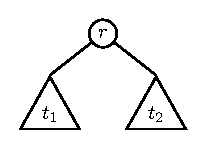
\includegraphics[bb=71 668 148 721]{non-empty_tree}
    \end{center}
  \column{0.5\textwidth}
    A depth-first traversal from left to right visits first node
    \id{r}, then the left subtree \id{t_1} and finally the right
    subtree \id{t_2}. But if we want to keep track of the visited
    nodes, we have several ways.
\end{columns}

\bigskip

\begin{itemize}

  \item We can record \id{r}, then nodes of \id{t_1} and finally
  nodes of \id{t_2}: this is \textbf{left prefix traversal};

  \item we can record nodes of \id{t_1}, then \id{r} and nodes of
  \id{t_2}: this is a \textbf{left infix traversal}; 

  \item we can record nodes of \id{t_1}, then nodes of \id{t_2} and
  finally \id{r}: this is a \textbf{left postfix traversal}.

\end{itemize}

\end{frame}

% ------------------------------------------------------------------------
%
\begin{frame}
\frametitle{Binary trees/Left prefix traversal}

Let us augment the specification \(\proc{Bin-tree}(\type{node})\)
with a new function realising a \textbf{left prefix traversal}. In
order to record the traversed nodes, we need an additional
structure. Let us take a stack and call our traversal
\proc{Lpref}. 

\bigskip

The additional signature is straightforward:
\[
\proc{Lpref} : 
\proc{Bin-Tree}(\type{node}).\type{t} \rightarrow
\proc{Stack}(\type{node}).\type{t}
\]
The corresponding equations are
{\small
\begin{align*}
   \proc{Lpref} (\proc{Empty}) 
&= \proc{Empty}\\
   \proc{Lpref} (\textbf{\proc{Make} (\id{e}, \id{t_1}, \id{t_2})}) 
&= \proc{Push} (\textbf{\id{e}},
   \proc{Append} (\proc{Lpref} (\textbf{\id{t_1}}), \proc{Lpref}
   (\textbf{\id{t_2}})))
\end{align*}
}
where we omitted the prefixes
``\proc{Bin-Tree}(\type{node})'' and ``\proc{Stack}(\type{node})''.

\end{frame}

% ------------------------------------------------------------------------
%
\begin{frame}
\frametitle{Binary trees/Left prefix traversal (cont)}

These equations must obviously be oriented from left to right:
{\small
\begin{align*}
   \proc{Lpref} (\proc{Empty}) 
&\rightarrow \proc{Empty}\\
   \proc{Lpref} (\proc{Make} (\id{e}, \id{t_1}, \id{t_2})) 
&\rightarrow \proc{Push} (\id{e}, \proc{Append} (\proc{Lpref}
   (\id{t_1}), \proc{Lpref} (\id{t_2})))
\end{align*}
}
where we omitted the specification prefixes.

\bigskip

This is a left to right traversal if the evaluation strategy computes
the value of arguments \emph{from left to right}.

\bigskip

\emph{It is important to distinguish between the moment when a node is
  encountered and when it is added in the resulting stack.} Therefore,
if the arguments of \proc{Lpref} are computed from right to left, the
traversal is from right to left, but the nodes in the final stack will
be ordered from left to right (as specified).

\end{frame}

% ------------------------------------------------------------------------
%
\begin{frame}
\frametitle{Binary trees/Left postfix traversal}

The additional signature for left postfix traversal is:
\[
\proc{Lpost} : 
\proc{Bin-Tree}(\type{node}).\type{t} \rightarrow
\proc{Stack}(\type{node}).\type{t}
\]
The corresponding equations are
{\small
\begin{align*}
\proc{Lpost} (\proc{Empty}) &= \proc{Empty}\\
\proc{Lpost} (\textbf{\proc{Make} (\id{e}, \id{t_1}, \id{t_2})}) &=\\
\proc{Append} (\proc{Lpost} (\textbf{\id{t_1}}),
     \proc{Append} (\proc{Lpost} (\textbf{\id{t_2}}), 
                    \proc{Push} (\textbf{\id{e}}, \proc{Empty})))
\end{align*}
}
where we omitted the specification prefixes.

\end{frame}

% ------------------------------------------------------------------------
%
\begin{frame}
\frametitle{Binary trees/Left postfix traversal (cont)}

We orient these equations from left to right:
{\small
\begin{align*}
   \proc{Lpost} (\proc{Empty}) 
&\rightarrow \proc{Empty}\\
   \proc{Lpost} (\proc{Make} (\id{e}, \id{t_1}, \id{t_2})) 
&\rightarrow\\
 \proc{Append} (\proc{Lpost} (\id{t_1}),
   \proc{Append} (\proc{Lpost} (\id{t_2}), \proc{Push} (\id{e},
   \proc{Empty})))
\end{align*}
}
where we omitted the specification prefixes.

\end{frame}

% ------------------------------------------------------------------------
%
\begin{frame}
\frametitle{Binary trees/Left infix traversal}

The additional signature for left infix traversal is simply:
\[
\proc{Linf} : 
\proc{Bin-Tree}(\type{node}).\type{t} \rightarrow
\proc{Stack}(\type{node}).\type{t}
\]
The corresponding equations are
\begin{align*}
   \proc{Linf} (\proc{Empty}) 
&= \proc{Empty}\\
   \proc{Linf} (\textbf{\proc{Make} (\id{e}, \id{t_1}, \id{t_2})}) 
&= \proc{Append} (\proc{Linf} (\textbf{\id{t_1}}), 
   \proc{Push} (\textbf{\id{e}}, \proc{Linf} (\textbf{\id{t_2}})))
\end{align*}
where we omitted the specification prefixes.

\end{frame}

% ------------------------------------------------------------------------
%
\begin{frame}
\frametitle{Binary trees/Left infix traversal (cont)}

We must orient these equations from left to right:
\begin{align*}
   \proc{Linf} (\proc{Empty}) 
&\rightarrow \proc{Empty}\\
   \proc{Linf} (\proc{Make} (\id{e}, \id{t_1}, \id{t_2})) 
&\rightarrow \proc{Append} (\proc{Linf} (\id{t_1}), 
   \proc{Push} (\id{e}, \proc{Linf} (\id{t_2})))
\end{align*}
where we omitted the specification prefixes.

\end{frame}

% ------------------------------------------------------------------------
%
\begin{frame}
\frametitle{Binary trees/Breadth-first traversal}

Let us consider the pictures of
page~\pageref{breadth_first_pictures}. 

\bigskip

The idea it that we need to find at each level the nodes belonging to
the next level, adding them to the previous nodes and repeat the
search. So we need to handle at each level a \textbf{forest}, i.e. a
set (or stack) of trees, not just nodes because nodes do not contain
the subtrees (thus the next level nodes).

\bigskip

Therefore let us add first a function to the signature of
\(\proc{Bin-tree}(\type{node})\):
\[
{\cal B} :
\proc{Stack}(\proc{Bin-tree}(\type{node}).\type{t}).\type{t}
\rightarrow \proc{Stack}(\type{node}).\type{t}
\]
such that expression \({\cal B}(\,\id{f})\) is a stack of the
nodes of forest \id{f} traversed in a breadth-first way from left to
right.

\bigskip

Let specify \(\proc{Forest}(\type{node}) = \proc{Stack}
(\proc{Bin-tree}(\type{node}).\type{t})\)

\end{frame}

% ------------------------------------------------------------------------
%
\begin{frame}
\frametitle{Binary trees/Breadth-first traversal (cont)}
\label{bfs}

Then we define a function 
\[\proc{BFS} : \proc{Bin-tree}(\type{node}).\type{t} \rightarrow
\proc{Stack}(\type{node}).\type{t}
\]
such that expression \(\proc{BFS}(\id{t})\) is a stack of the nodes of
the tree \id{t} traversed in a breadth-first way from left to
right. The corresponding equation is simply
\[
\proc{BFS} (\id{t}) = {\cal B}
(\proc{Stack}(\type{node}).\proc{Push} (\id{t}, \proc{Empty}))
\]
Now, in order to define \({\cal B} (\,\id{f})\) we need to get
\begin{itemize}

  \item the roots of the forest \,\id{f},

  \item the forest rooted at level 1 of the forest \,\id{f}.

\end{itemize}

\end{frame}

% ------------------------------------------------------------------------
%
\begin{frame}
\frametitle{Binary trees/Breadth-first traversal (cont)}
\label{roots}

Let \proc{Roots} have the signature
\[
\proc{Roots} : \proc{Forest}(\type{node}).\type{t} \rightarrow
\proc{Stack}(\type{node}).\type{t}
\]
The corresponding equations are not difficult to guess:
\begin{align*}
   \proc{Roots} (\proc{Forest}(\type{node}).\proc{Empty}) 
&= \proc{Stack} (\type{node}).\proc{Empty}\\
   \proc{Roots} (\proc{Push} (\proc{Empty}, \,\id{f}))
&= \proc{Roots} (\,\id{f})\\
   \proc{Roots} (\proc{Push} (\proc{Make} (\id{r}, \id{t_1},
   \id{t_2}), \,\id{f}))
&= \proc{Push} (\id{r}, \proc{Roots} (\,\id{f}))
\end{align*}
These equations must be oriented from left to right (do you see
why?).

\end{frame}

% ------------------------------------------------------------------------
%
\begin{frame}
\frametitle{Binary trees/Breadth-first traversal (cont)}
\label{next_level}

We have to define now a function which, given a forest, returns the
forest at level 1, i.e. all the subtrees rooted at level 1 for each
tree in the initial forest. Let us call it 
\[
\proc{Next} : \proc{Forest}(\type{node}).\type{t} \rightarrow
\proc{Forest}(\type{node}).\type{t} 
\]
The equations are 
\begin{align*}
   \proc{Next} (\proc{Forest}(\type{node}).\proc{Empty}) 
&= \proc{Forest} (\type{node}).\proc{Empty}\\
   \proc{Next} (\proc{Push} (\proc{Empty}, \,\id{f}))
&= \proc{Next} (\,\id{f})\\
   \proc{Next} (\proc{Push} (\proc{Make} (\id{r}, \id{t_1},
   \id{t_2}), \,\id{f}))
&= \proc{Push} (\id{t_1}, \proc{Push} (\id{t_2}, \proc{Next}
   (\,\id{f})))
\end{align*}
Note the similarities between \proc{Next} and \proc{Roots}. Note
also that \id{t_1} and \id{t_2} may be \proc{Empty}, for the sake of
simplicity.

\end{frame}

% ------------------------------------------------------------------------
%
\begin{frame}
\frametitle{Binary trees/Breadth-first traversal (cont)}
\label{forest_bfs}

Now we can write the equations of \({\cal B}\), using
\proc{Roots} and \proc{Next}:
\begin{eqnarray*}
  {\cal B} (\proc{Forest}(\type{node}).\proc{Empty})
= \proc{Stack}(\type{node}).\proc{Empty}\\
  {\cal B} (\,\textbf{\id{f}})
= \proc{Append} (\proc{Roots} (\,\id{f}), {\cal B}
  (\textbf{\proc{Next} (\,\id{f})}))
\end{eqnarray*}
where \(\id{f} \neq \proc{Empty}\).

\bigskip

Match the traversal as defined formally here against a figure
page~\pageref{breadth_first_pictures}.

\bigskip

Let us orient these equations from left to right. 

\bigskip

In order to show that the resulting rewriting system terminates, we
have to compare the height of the \emph{values} of \,\id{f} and
\(\proc{Next} (\,\id{f})\).

\end{frame}

% ------------------------------------------------------------------------
%
\begin{frame}
\frametitle{Binary trees/Breadth-first traversal (cont)}

The intuition is that expression \(\proc{Next} (\,\id{f})\)
denotes a \emph{larger} forest than \,\id{f}, because it is made of
the direct subtrees of \,\id{f} (if they are all non-empty, then we
get twice as more trees than in \,\id{f}), but the trees are strictly
\emph{smaller}.

\bigskip

Since we traverse the levels in increasing order, theses trees will
finally be empty. But the second equation discards empty trees, so in
the end, we really get an empty forest.

\bigskip

With this reasoning we show that the terminating orientation is
\begin{align*}
   \proc{Next} (\proc{Forest}(\type{node}).\proc{Empty}) 
&\rightarrow \proc{Forest} (\type{node}).\proc{Empty}\\
   \proc{Next} (\proc{Push} (\proc{Empty}, \,\id{f}))
&\rightarrow \proc{Next} (\,\id{f})\\
   \proc{Next} (\proc{Push} (\proc{Make} (\id{r}, \id{t_1},
   \id{t_2}), \,\id{f}))
&\rightarrow \proc{Push} (\id{t_1}, \proc{Push} (\id{t_2}, \proc{Next}
   (\,\id{f})))
\end{align*}

\end{frame}
